%&pdflatex
\documentclass[11pt]{article}
\usepackage{url,enumerate, amssymb, amsfonts}
\usepackage[colorlinks = true,
linkcolor = blue,
urlcolor  = blue,
citecolor = green,
anchorcolor = blue]{hyperref}
%\usepackage{setspace,listings}
\usepackage{graphicx}
\usepackage{amsmath}
\usepackage{psfrag}
\usepackage[font=small,labelfont=bf]{caption}
\usepackage{enumerate}
\usepackage{authblk}
\usepackage[sort&compress,comma,square,numbers]{natbib}
\usepackage{url} % not cruci
%\pdfminorversion=4
\usepackage{setspace}
\usepackage{lscape}
\usepackage{color,amssymb}
\usepackage{mathtools}
\usepackage{dcolumn}
\usepackage{indentfirst, verbatim, float}
\usepackage[margin=0.82in]{geometry}
%\newcounter{equationset, sectsty, breqn}
%\usepackage{setspace, amsmath,color}
%\usepackage{color,amssymb}
\usepackage{mathtools, amsthm, subcaption}
\theoremstyle{definition}
\newtheorem{definition}{Definition}[section]
\newtheorem{theorem}{Theorem}[section]
\newtheorem{corollary}{Corollary}[theorem]
\newtheorem{lemma}[theorem]{Lemma}
\newtheorem{remark}{Remark}
\bibliographystyle{plainnat}
\usepackage{sidecap}
\usepackage{titlesec}
\sidecaptionvpos{figure}{c}

% NOTE: To produce unblinded version, replace "0" with "1" below.
\newcommand{\blind}{0}
% DON'T change margins - should be 1 inch all around.

\begin{document}

\def\spacingset#1{\renewcommand{\baselinestretch}%
{#1}\small\normalsize} \spacingset{1}

%%%%%%%%%%%%%%%%%%%%%%%%%%%%%%%%%%%%%%%%%%%%%%%%%%%%%%%%%%%%%%%%%%%%%%%%%%%%%%
\title{\bf Testing independence in networks via family of network metrics}
\if1\blind
{\author[1]{Youjin Lee (ylee160@jhu.edu)} %\thanks{cshen6@jhu.edu}}
	\author[2]{Cencheng Shen} %\thanks{cshen6@jhu.edu}}
	\author[2,3,4]{Joshua T. Vogelstein}
	\affil[1]{Department of Biostatistics, Johns Hopkins University}
  \affil[2]{Center for Imaging Science, Johns Hopkins University}
  \affil[3]{Department of Biomedical Engineering and Institute for Computational Medicine, Johns Hopkins University}
  \affil[4]{Institute for Data-Intensive Engineering \& Science, Johns Hopkins University}
	\maketitle
} \fi

	\if0\blind
	{
		\bigskip
		\bigskip
		\bigskip
		\begin{center}
			{\LARGE\bf Testing independence in networks via family of network metrics}
		\end{center}
		\medskip
	} \fi

\begin{abstract}
%The text of your abstract. 200 or fewer words.
Investigating how network structures are associated with nodal attributes of interest is a core problem in network science. As the network topology is a structured and often high-dimensional object, many traditional nonparametric tests are no longer applicable and parametric approaches are dominant in graph inferences. Here we propose a new procedure to testing dependence between graphs and attributes, via diffusion distances and distance-based correlation testing. We demonstrate that our nonparametric method not only yields a consistent test statistic under common network models, but also significantly surpasses the testing power of existing benchmarks under various circumstances. 
\end{abstract}

\noindent%
{\it Keywords:} network dependence, distance correlation, exchangeable graph, diffusion maps

\sloppy
\doublespacing

\section{Introduction}
\label{sec:intro}
	\vspace*{-0.2cm}
	% General Backgrounds
Propelled by increasing demand and supply of graph data from various disciplines, the ubiquitous influence of network inferences has motivated numerous recent advances and applications in statistics, physics, computer science, biology, social science, etc., which further poses many new challenges to data scientists. One of the most fundamental statistical question is to determine and characterize the relationship among multiple modalities of a given data set, for which the first step is to test the existence of any dependency. However, the lack of a principal notion of correlation in the graph domain has not only hindered the progress of nonparametric dependency testing methods, but also deterred a rich literature of statistical techniques in other inferences (e.g., regression, feature screening, two-sample test) from being directly applied to graphs.
 
% Testing dependence
Statisticians have long considered the problem of revealing the relationship between two data sets. The most classical approach is the Pearson's correlation (\cite{Pearson1895}), which determine the existence of linear relationship via a correlation coefficient in the range of $[-1,1]$, with $0$ indicating no linear association while $\pm 1$ indicating perfect linear association. To capture all types of dependencies not limited to linear relationship, many new correlation measures and nonparametric statistics have been suggested to test independence between two random vectors~\citep{mantel1967, RobertEscoufier1976, szekely2007measuring, GrettonGyorfi2010, Reshef2011, HellerGorfine2013,szekelyRizzo2013a, heller2016consistent, shen2016discovering}. In particular, the distance correlation by Szekely et al. \citep{szekely2007measuring} is the first correlation measure that is consistent against all possible dependencies (with finite moments), and the multiscale generalized correlation (MGC) statistic by Shen et al. \cite{shen2016discovering} inherits the same consistency of distance correlation with significantly better finite-sample testing powers under high-dimensional and nonlinear dependencies, via defining a family of distance-based local correlations and efficiently searching the optimal correlation for testing.

% Graph data general
Despite of many recent development, the network data, different from a random vector, still suffers from a dearth of proper analysis, due to its structured and high-dimensional nature. Mathematically, a graph $G=(V,E)$ consists of a set $V$ of nodes (or vertices) together with a set $E$ of edges, which is often represented via an adjacency matrix $A = \{A_{ij} : i,j= 1,..,n \}$, e.g. for an unweighted and undirected network, $A_{ij} = 1$ if node $i$ and node $j$ are connected by an edge, and zero otherwise. Therefore, $A$ is a symmetric square matrix that does not satisfy traditional data assumptions, e.g., each observation can be assumed independently and identically distributed, the sample size increases faster than the feature dimension, etc., which is a huge obstacle for directly applying conventional statistical methods. 

% testing dependence on graphs
When it comes to investigating relationships in network data, a core problem is to detect dependency between network topology and nodal attributes, i.e., certain properties defined on nodes. For example, each person on Facebook having a number of different attributes, e.g., occupations, sex, personal behaviors, etc., are interacting each other via the social network; in neuro-science, each brain region has its own functionality, but is connected with other regions in the brain map. Identifying dependency between network and nodal attributes has primarily focused on their relationship explained only by network model under the boundary of model assumption \citep{wasserman1996logit, howard2016understanding, fosdick2015testing}. Even though Fosdick and Hoff \cite{fosdick2015testing} suggested estimating node-specific network factors without restricting the dimensions, a fundamental difficulty of model-based independence tests still lingers from the fact that not all networks exhibit the structures described by known network models. To our best knowledge so far, there is no principled method to compute a model-free correlation measure for testing network dependency. 

%Most network analysis starts with a proper model, i.e., latent position model, stochastic block model, random dot product model \citep{HollandEtAl1983, YoungScheinerman2007,RoheEtAl2011,karrer2011stochastic,ZhaoLevinaZhu2012,SussmanEtAl2012,TangSussmanPriebe2013}
% proposed solution
To overcome the obstacles due to the distinct structure of network data and also due to the limitations of model-based method, we first define a family of distance metrics on network data via the diffusion maps, then apply nonparametric testing method of MGC utilizing the diffusion distance of the network topology and the Euclidean distance of the nodal attributes. Theoretical results show that under very mild condition, the diffusion maps, acting as a node-specific random vector, can allow distance-based correlation measures to be consistent in testing network dependencies. Moreover, the MGC statistic offers major power improvement under various scenarios in finite-sample testing. We further illustrate the advantages of diffusion maps and MGC over the existing benchmarks via comprehensive simulations under popular network models.

% literature reviews about testing network independence. 

% specify the goal / approach of our research and explain the outline 
%Different from a random vector, network or equivalently graph involves a particular construction which we should take into account. Throughout this paper, we assume that we are given an unweighted and undirected network without self-loop, comprised of $n (\in \mathbb{N})$ nodes. An adjacency matrix of this given network, denoted by $\mathbf{A} = \{A_{ij} : i,j= 1,..,n \}$, is to formalize the relational data of network, where $A_{ij} = 1$ if node $i$ and node $j$ are adjacent each other and zero otherwise. Let us define a $m$-variate ($m \in \mathbb{N}$) random variable associated with each node, i.e. nodal attributes, $\mathbf{X}  \in \mathbb{R}^{m}$ which we are interested in. We first have to consider increasing amount of information inherent in network data as the number of nodes increases, which might lead to diverse patterns in dependency as well. In addition, by its definition, an adjacency matrix $\mathbf{A}$ inherits dependency among its columns and rows, so thus it cannot enjoy the traditional setting based on a random vector. To overcome these challenges, we propose applying distance-based statistic called multiscale generalized correlation (\texttt{MGC})~\citep{shen2016discovering} into testing network independnece along with the network geometries derived from random walk on graph. We are going to elaborate the statistic and demonstrate its validity for a family of graphs in Section~\ref{sec:method}. In Section~\ref{sec:simulation}, simulation results demonstrate the best performance of our method compared to the existing under various circumstances.
	\vspace*{-0.2cm}
\section{Results}
\label{sec:method}
	\vspace*{-0.2cm}
\subsection{Family of Network Independence Test Statistics}
\label{ssec:method2}

In order to satisfy the requirement of being \textit{i.i.d}, we are going to restrict applicable network to a certain family of graphs and suggest valid graph geometries that furnish us useful metrics. A graph $\mathbf{G}$ is called exchangeable if and only if its adjacency matrix $\mathbf{A}$ is jointly exchangeable \citep{orbanz2015bayesian}, i.e.~for every permutation $\sigma$ of $n$, $(A_{ij}) \stackrel{d}{=} (A_{\sigma(i) \sigma(j)})$. Even though exchangeability itself cannot guarantee being \textit{i.i.d}, thanks to the \textit{de Finetti}'s representation theorem and \textit{Aldous-Hoover theorem}, exchangeable graph, often called \textit{graphon} \citep{lovasz2006limits}, can be defined through conditionally \textit{i.i.d} edge distribution \citep{chan2013estimation}. We then take advantage of this \textit{i.i.d} expression which draws \textit{i.i.d} network geometries called \textit{diffusion maps}.

\begin{figure}[ht]
	\centering
	\begin{subfigure}[b]{0.23\textwidth}
		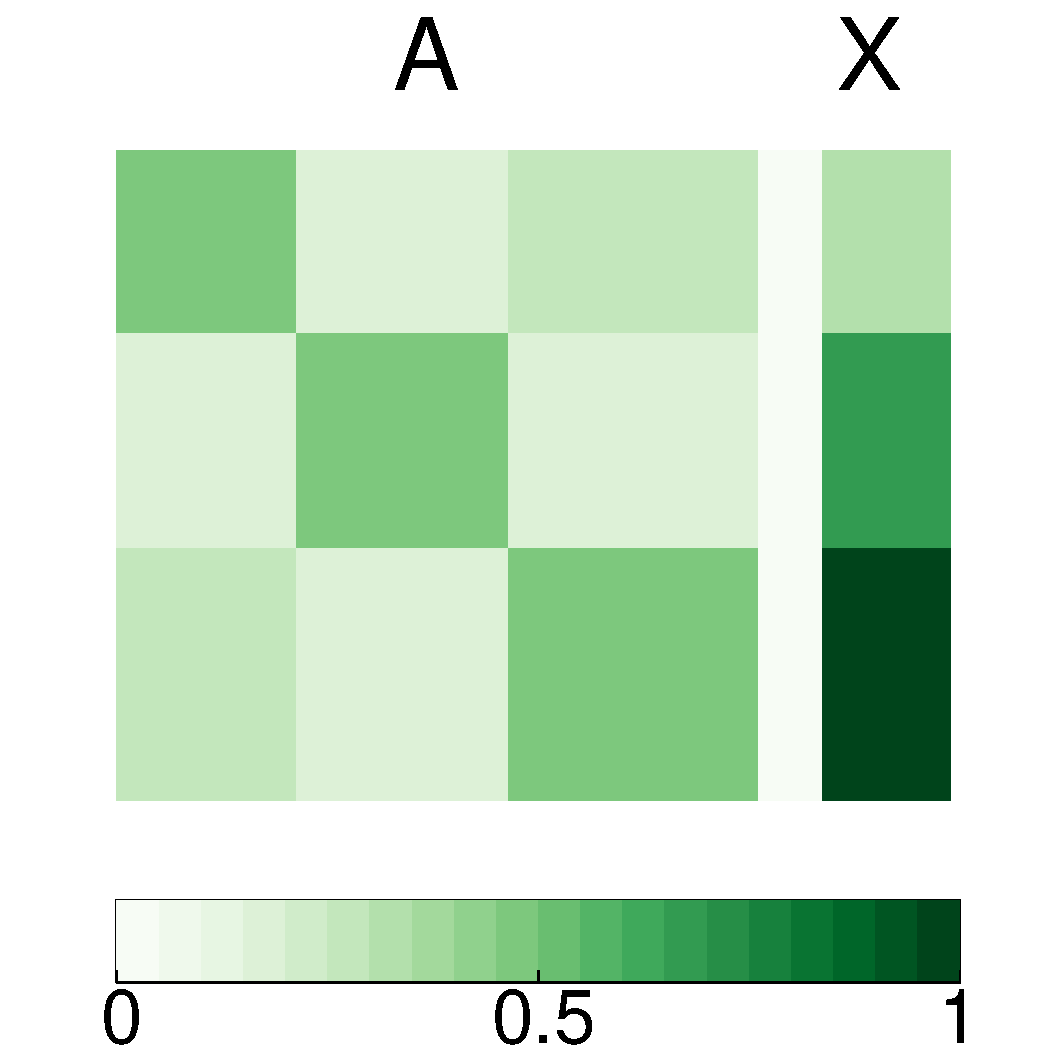
\includegraphics[width=\textwidth]{../Figure/Pmat.pdf}
		\caption{}
		\label{fig:a}
	\end{subfigure}
	~ %add desired spacing between images, e. g. ~, \quad, \qquad, \hfill etc. 
	%(or a blank line to force the subfigure onto a new line)
	\begin{subfigure}[b]{0.23\textwidth}
		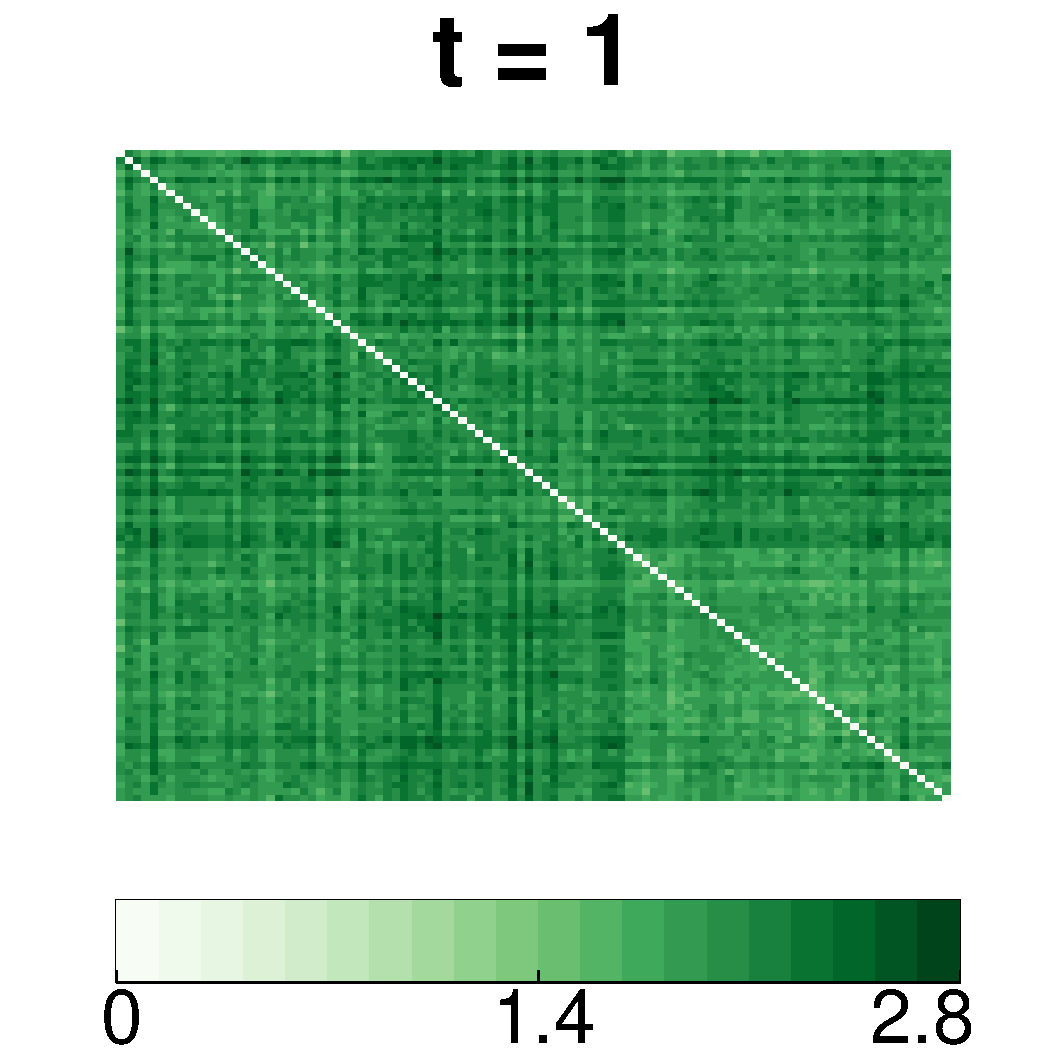
\includegraphics[width=\textwidth]{../Figure/Dx1.pdf}
		\caption{}
		\label{fig:b}
	\end{subfigure}
	~ %add desired spacing between images, e. g. ~, \quad, \qquad, \hfill etc. 
	%(or a blank line to force the subfigure onto a new line)
	\begin{subfigure}[b]{0.23\textwidth}
		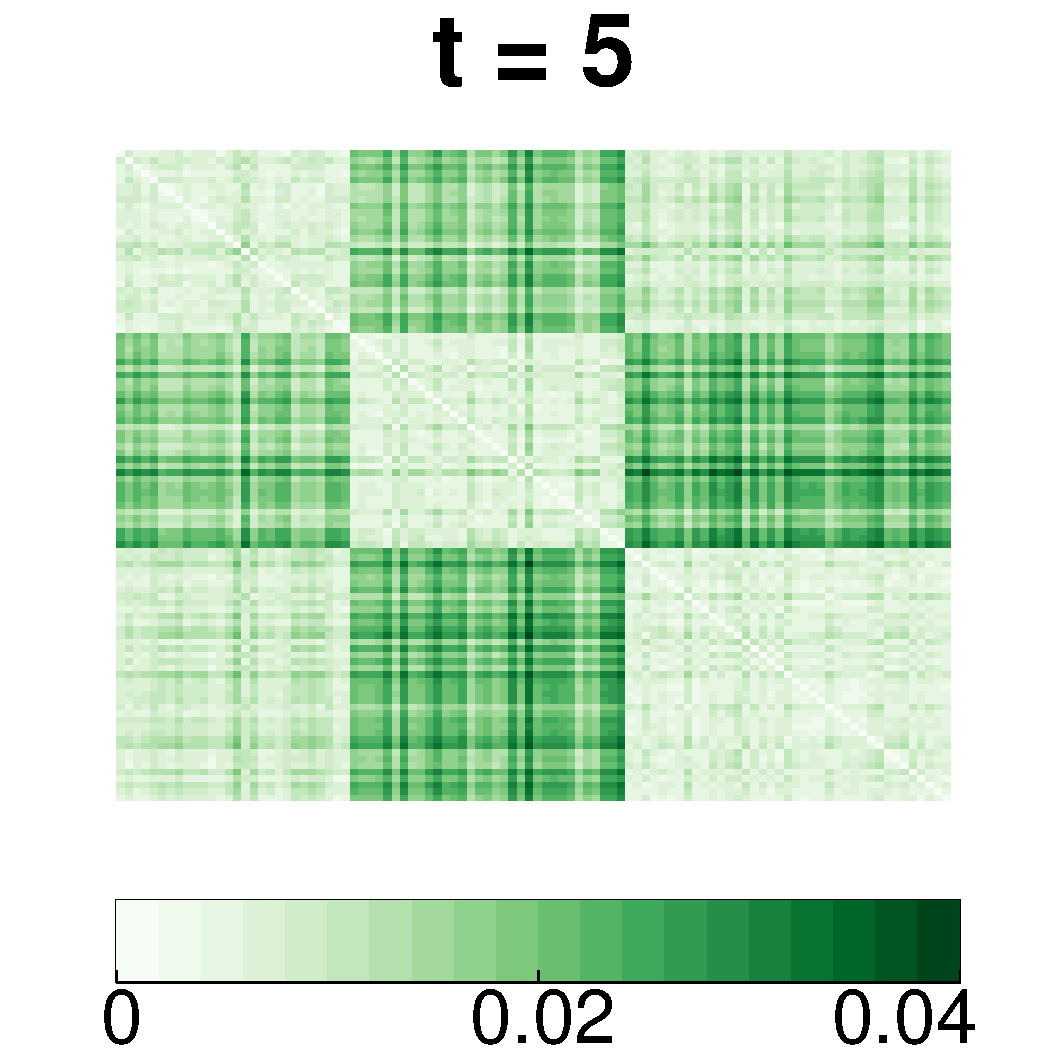
\includegraphics[width=\textwidth]{../Figure/Dx5.pdf}
		\caption{}
		\label{fig:c}
	\end{subfigure}
	\begin{subfigure}[b]{0.23\textwidth}
		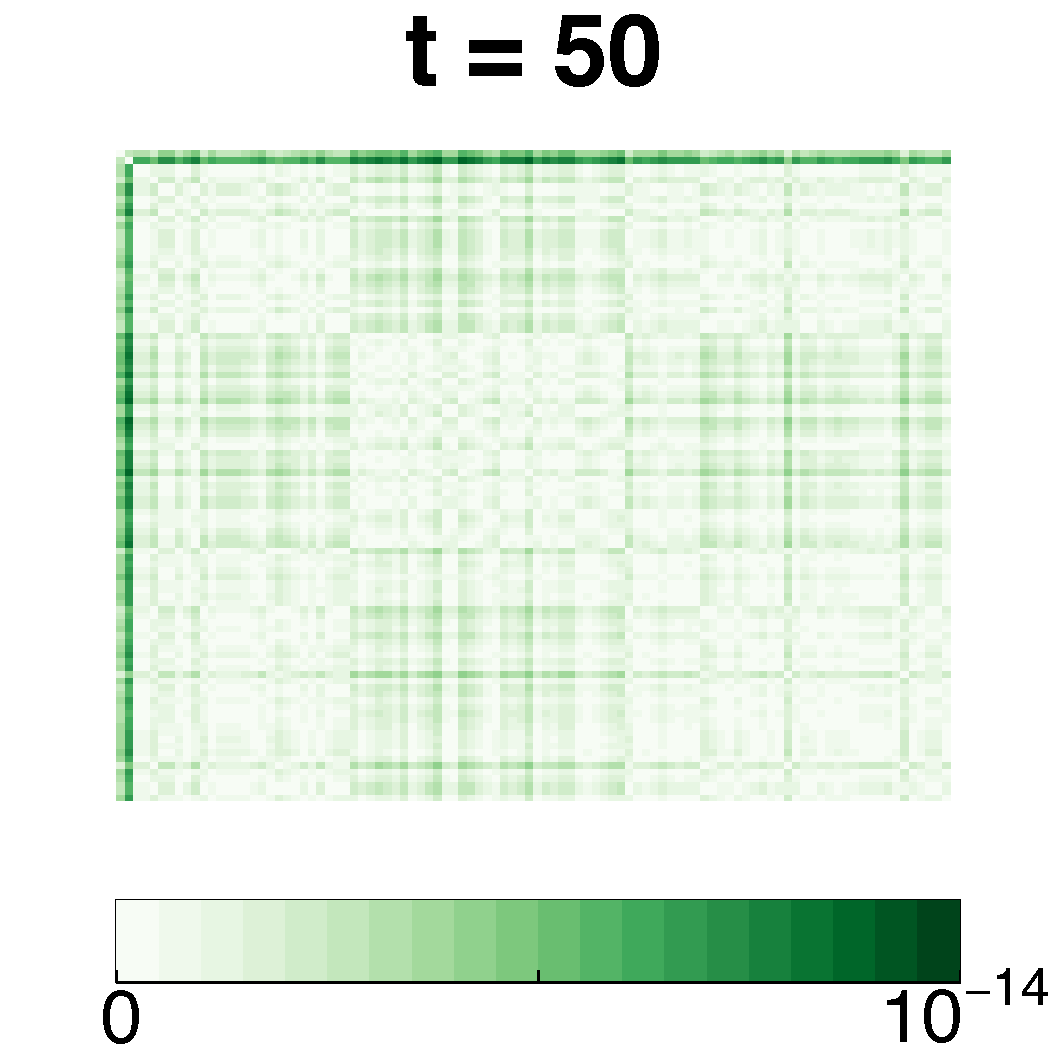
\includegraphics[width=\textwidth]{../Figure/Dx50.pdf}
		\caption{}
		\label{fig:d}
	\end{subfigure}
	\caption{Figure (a) shows data generating probability of an adjacency matrix $\mathbf{A}$ and nodal attributes $\mathbf{X}$. Diffusion matrix, as a proposed network metric, provides one-parameter family of network-based distances where as time goes by the pattern shown in the distance matrix changes, and at time point $t = 5$, distance matrix (c) illustrates most clear block structures and at the same time it exhibits most dependence to distance matrix of $\mathbf{X}$.}
	\label{fig:diffusions}
\end{figure}
\cite{coifman2006diffusion} proposed diffusion maps as a meaningful multiscale geometries which is defined by eigenvectors of Markov matrix constructed over a connected network. In the process of constructing such Markov matrix, we basically run random walks by iterating transition matrix and diffusion maps accordingly locates each node's position at each iteration time. Distance between each pair of nodes, defined as a \textit{diffusion distance}, then can be derived from an Euclidean distance of such diffusion maps. Each of diffusion distance, i.e.~$C_{t}$, can also be represented using a discrete set of real nonzero eigenvalues $\{ \lambda_{r} \}$ and eigenvectors $\{ \phi_{r}  \}$ of a transition matrix~\citep{coifman2006diffusion,lafon2006diffusion}. 
\begin{equation}
\label{eq:diffusion}
C^2_{t}[i,j]  :=   \parallel \mathbf{U}_{t}(i) - \mathbf{U}_{t}(j) \parallel   \quad i,j = 1,2, \ldots , n,
\end{equation}
where $\mathbf{U}_{t}(i) = \begin{pmatrix} \lambda^{t}_{1} \phi_{1}(i) & \lambda^{t}_{2} \phi_{2} (i)  & \ldots & \lambda^{t}_{q} \phi_{q}(i) \end{pmatrix}^{T} \in \mathbb{R}^{q}$ is a diffusion map at time $t$. As diffusion time $t$ increases, distance matrix $C_{t}$ is more likely to take into account distance between two nodes which are relatively difficult to reach each other. Figure~\ref{fig:diffusions} shows three exemplary distance matrices among whole one-parameter family of distance $\{ C_{t} : t \in \mathbb{N} \}$. Compared to adjacent relation or geodesic distance which are two extremes, diffusion distance well reflects the connectivity since it takes into account every possible path between the two nodes. We prove that each diffusion map provides \textit{i.i.d} multivariate coordinates for each node under jointly exchangeable graph. Lemma~\ref{main_lemma} below provides us with \textit{i.i.d} one-parameter family of $\{ \mathbf{U}_{t} \}_{t \in \mathbb{N}}$. 
\begin{lemma}[Exchangeability and \textit{i.i.d} of diffusion maps $\mathbf{U}_{t}$]
	\label{main_lemma}
	Assume that a connected, undirected and unweighted graph $\mathbf{G}$ is an exchangeable random graph. Then its transition probability so thus diffusion maps at fixed time $t$ is also exchangeable, conditioned on underlying distribution of graph. Furthermore, by \textit{de Finetti's Theorem}, such diffusion maps at $t$, $\mathbf{U}_{t}(i) = \begin{pmatrix} \lambda^{t}_{1} \phi_{1}(i) & \lambda^{t}_{2} \phi_{2} (i)  & \ldots & \lambda^{t}_{q} \phi_{q}(i) \end{pmatrix}^{T}$, are conditionally \textit{i.i.d} given its underlying distribution.   
\end{lemma}

If a set of diffusion distances are applicable as a proper Euclidean distance in a distance-based test statistic~\ref{eq:dCov}, we are able to dispense with obstacles in testing network independence. First of all in a general setting, assume that we have a finite sample of infinitely exchangeable sequence $(\mathbf{W}, \mathbf{Y}) = \{  (\mathbf{w}_{i}, \mathbf{y}_{i} ) ; i = 1,2, \ldots, n \}$, which is identically distributed as $(\mathbf{w},\mathbf{y})$ with finite second moment.

\begin{theorem}
	Suppose that we are given $n$ pairs of exchangeable observations $(\mathbf{W}, \mathbf{Y}) = \{  (\mathbf{w}_{i}, \mathbf{y}_{i} ) ; i = 1,2, \ldots, n \}$ having finite second moment. Assume $\mathbf{w}_{i} \overset{i.i.d}{\sim} f_{\mathbf{w}}$ and $\mathbf{y}_{i} \overset{i.i.d}{\sim} f_{\mathbf{y}}$ given underlying distribution for $i = 1,2, \ldots, n$. Then
	\begin{eqnarray}
	\mathcal{V}_{n}^{2}(\mathbf{W},\mathbf{Y}) &\longrightarrow 0 \quad \mbox{ as } n \rightarrow \infty
	\end{eqnarray}	
	\textit{if and only if} $\mathbf{w}$ is independent of $\mathbf{y}$. Moreover, \texttt{dCorr} (\texttt{mCorr}) and \texttt{MGC} are consistent for testing dependence between $\mathbf{w}$ and $\mathbf{y}$, i.e., the testing power converges to $1$ asymptotically for any dependency of finite second moment.
	\label{theoremMain}
\end{theorem}

Note that if $\{ \mathbf{w}_{i} : i = 1,2,\ldots, n \}$ are \textit{i.i.d}, they are also exchangeable. Thus estimated latent network factors, which are assumed \textit{i.i.d} by \cite{fosdick2015testing} can also be applied to Theorem~\ref{theoremMain}. We already have shown that even under undirected network, diffusion maps remain exchangeable at each diffusion time point $t$. 

\begin{theorem}
	\label{theorem2}
	For $n$-pair of diffusion map and \textit{i.i.d} nodal attributes $\{ ( \mathbf{u}_{t}(i),  \mathbf{x}_{i}  ) : i =1,2, \ldots , n \}$ in a jointly exchangeable graph $\mathbf{G}$, we have $\mathbf{u}_{t}(i) \overset{i.i.d}{\sim} f_{U^{(t)}}$ and $\mathbf{x}_{i} \overset{i.i.d}{\sim} f_{\mathbf{X}}$ conditioned on underlying distribution of graph. 
	Then \texttt{MGC} is consistent in testing network independence with null of $H_{0}: f_{\mathbf{U}^{(t)} \cdot \mathbf{X}  }  = f_{\mathbf{U^{(t)}}} \cdot f_{\mathbf{X}}$. In particular, the consistency also holds for using the estimated latent network factors~\citep{fosdick2015testing} or an adjacency matrix of directed network as a distance matrix.
\end{theorem}

	\vspace*{-0.4cm}
\subsection{Distance-based Independence Test}
\label{ssec:method1}
% introduce standard 

\cite{szekely2007measuring} proposed a distance-based statistic having a marvelous closed form called distance correlation (\texttt{dCorr}). This distance-based multivariate independence test starts from the assumption that we are given $n \in \mathbb{N}$ pairs of \textit{i.i.d} random vectors $\big(  \mathbf{W}, \mathbf{Y}  \big)  = \{ (\mathbf{w}_{i}, \mathbf{y}_{i}) : \mathbf{w}_{i} \in \mathbb{R}^{q}; \mathbf{y}_{i} \in \mathbb{R}^{m}; i = 1,...,n \}$. Define distance matrices of $C_{ij} = \parallel \mathbf{w}_{i} - \mathbf{w}_{j} \parallel$ and $D_{ij} = \parallel \mathbf{y}_{i} - \mathbf{y}_{j} \parallel$ for $i,j=1,2, \ldots ,n$, where $\parallel \cdot \parallel$ indicates Euclidean distance.
Distance correlation (\texttt{dCorr}) is defined via distance covariance (\texttt{dCov}) $\mathcal{V}^2_{n}$ of $\mathbf{W}$ and $\mathbf{Y}$, which is the following: 
\begin{equation}	 
\label{eq:dCov}
\mathcal{V}^2_{n}(\mathbf{W}, \mathbf{Y}) = \frac{1}{n^2} \sum\limits_{i,j=1}^{n} \tilde{C}_{ij} \tilde{D}_{ij},
\end{equation}
where $\tilde{C}$ and $\tilde{D}$ is doubly-centered $C$ and $D$ by its column mean and row mean respectively. A modified distance covariance (\texttt{mCov}) and a modified distance correlation (\texttt{mCorr}) for testing high dimensional random vectors were also proposed in \cite{szekely2013distance}. However, neither \texttt{dCorr} nor ever \texttt{mCorr} still performs very well in the existence of various nonlinear dependency and under the existence of outliers as well~\citep{shen2016discovering}. Out of this concern, \cite{shen2016discovering} proposed Multiscale Generalized Correlation (\texttt{MGC}) via adding local scale in a sense of nearest neighbors on correlation coefficients. Multiscale version of distance covariance $\{ { {\mathcal{V}^{*}}^2_{n} }   \}_{kl}$ is defined as following : 
\begin{equation}
\label{eq:MGC}
{\mathcal{V}^{*}}^2_{n} (\mathbf{W}, \mathbf{Y})_{kl} = \frac{1}{n^2} \sum\limits_{i,j=1}^{n} \tilde{C}_{ij} \tilde{D}_{ij} I \big( r(C_{ij}) \leq k \big) I \big( r(D_{ij}) \leq l  \big) \quad k,l=1,2,..., n ,
\end{equation}
where $r(C_{ij})$ ($r(D_{ij})$) denotes a rank of $\mathbf{w}_{i}$ ($\mathbf{y}_{i}$) relative to $\mathbf{w}_{j}$ ($\mathbf{y}_{j}$), i.e.~$r(C_{ij}) = k$ means $w_{i}$ is $w^{'}_{j}$s $k$-nearest neighbor. Based on this set of statistics, \texttt{MGC} finds the \textit{best statistic} which exhibits the largest correlation between the two data sets without inducing multiple testing problems. It has already been shown that this local scaled statistic performs no worse than \texttt{dCorr} and that it actually results in improved sensitivity to nonlinear dependence than \texttt{dCorr}. 

Now back to the network independence test, we are ready to derive the Euclidean distance of $\mathbf{X}$, e.g. $D$; while how to construct the distance matrix corresponding to network structure is still questionable. We are required \textit{i.i.d} node-specific coordinates of which Euclidean distance as $C$ in statistics~\ref{eq:MGC} reflects a network-based distance between nodes. We can first conjecture directly using an Euclidean distance of an adjacency matrix $\mathbf{A}$. The Euclidean distance from each column of adjacency matrix, however, may not satisfy the requirement for consistency since columns of $\mathbf{A}$ are often dependent each other.

\subsection{Measure for Node Contribution}
On the other hand, some nodes often exert more reliance on their attributes than the others. Here we suggest the measure of node's contribution to detecting dependence as a byproduct of \texttt{MGC} statistic. Let $(k^{*}, l^{*})$ be the optimal neighborhood choice in distance matrix $(C, D)$ respectively. Denote the contribution of node $v \in V(G)$ to the testing statistic by  $c(\cdot) : v \rightarrow \mathbb{R}$
\begin{equation}
\label{eq:contribution}
c(v) \propto \sum\limits_{j=1}^{n} \tilde{C}_{j v} \tilde{D}_{j v} I \big(  r (C_{j v}) \leq k^{*}  \big) I \big( r (D_{ j v }) \leq l^{*} \big), 
\end{equation}
which is proportional to $v^{th}$ column-sum of the pre-summed test statistic~\ref{eq:MGC}. Note that the deviation of non-negative \texttt{MGC} statistic from zero implies departure from the independence and also note that we truncate the correlation in \texttt{dCov} by column entry's rank. Thus $\tilde{C}_{jv} \tilde{D}_{jv}$ would not be truncated if node $j$ $(\in \{ 1,2, \ldots, n \} \setminus \{v \} )$ is important to node $v$ and its larger, positive value would contribute to ${\mathcal{V}^{*}_{n}}^2$ more. The statistic $c(v)$ comes out from these observations. 

%%%%%%%%%%%%%%%%%%%%%%%%%%%%%%%%%%%%%%%%%%%%%%%%%%
\section{Simulation Study}
\label{sec:simulation}
	\vspace*{-0.2cm}
In our simulation studies, we make a comparison between empirical testing power between \texttt{MGC}, \texttt{mCorr}, Heller-Heller-Gorfine (\texttt{HHG}) \citep{heller2012consistent}, and likelihood ratio test of Fosdick and Hoff (\texttt{FH})~\citep{fosdick2015testing}. We use type I error of $\alpha = 0.05$ and obtain p-values from each simulated network via permutation test. All the simulation models can be illustrated by joint distribution of adjacent matrix $\mathbf{A}$ and nodal attributes $\mathbf{X}$. We introduced a popular network model of Stochastic Block Model (SBM) as our main simulated networks. 

\subsection{Stochastic Block Model}

\begin{SCfigure}[][h]
	\centering
	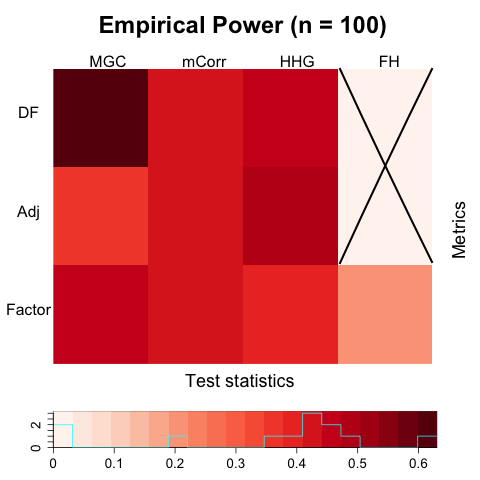
\includegraphics[width=0.4\paperwidth, height=0.4\paperwidth]{../Figure/ThreeSBM_results_simple.png}
	\caption{This power heatmap illustrates the superior power of multiscale generalized correlation (\texttt{MGC}) under diffusion distance matrix (\texttt{DF}) in three SBM (model~\ref{eq:Three}), compared to under adjacency matrix distance (\texttt{Adj}) or latent factor distance (\texttt{LT}). This demonstrates one exemplary network where \texttt{MGC} statistic along with a family of diffusion distances catches non monotonic correlations efficiently than the other statistics and metrics.}
	\label{fig:threeSBM}
\end{SCfigure}
We present the SBM with $K=3$ blocks (model~\ref{eq:Three}) where block affiliation for each node is correlated with its attributes $X$. Figure~\ref{fig:threeSBM} illustrates superior performance of \texttt{MGC} as a test statistic combined with diffusion maps (\texttt{DF}) as a network metric. Assume that for $i,j = 1, \ldots , n = 100$, we have
\begin{equation}
\label{eq:Three}
E(A_{ij} | X_{i}, X_{j}) = 0.5 I(|X_{i} - X_{j}| = 0) + 0.2 I(|X_{i} - X_{j}| = 1) + 0.3 I(|X_{i} - X_{j}| = 2), 
\end{equation}
where $X_{i} \overset{i.i.d}{\sim} Multiple(1/3, 1/3, 1/3); i = 1, \ldots, 100$. When $X_{i} = X_{j}$, these two nodes are most likely to have an edge but when $X_{i}$ and  $X_{j}$ differ by one, they are even less likely to have an edge, with probability of 0.2, than the most different pairs of nodes. This actually describes nonlinear dependence where \texttt{MGC} is believed to work better than the distance correlation. To scrutinize our conjecture on better performance of local optimal scaled \texttt{MGC} over global scale of \texttt{mCorr}, we control the amount of \textit{nonlinear dependency} through changing the value of $\theta \in (0, 1)$ in the three block model~\ref{eq:mono}. 
\begin{equation}
E(A_{ij} | X_{i}, X_{j}) = 0.5 I(|X_{i} - X_{j}| = 0) + 0.2 I(|X_{i} - X_{j}| = 1) + \theta I(|X_{i} - X_{j}| = 2), \quad i,j = 1, \ldots, n = 100, 
\label{eq:mono}
\vspace*{-0.4cm}
\end{equation}
where  $X_{i} \overset{i.i.d}{\sim} Bern(0.5); i =1, \ldots, 100$. When $\theta > 0.2$, linear dependency of edge distribution in $\mathbf{A}$ upon nodal attribute of $X$ is lost. If you see Figure~\ref{fig:powerplot}, power of \texttt{mCorr} starts to drop from $\theta = 0.2$ while that of \texttt{MGC} almost stays clam, which implies \texttt{MGC} is significantly more sensitive to nonlinear dependency compared to \texttt{mCorr}.  
\begin{figure}[ht]
	\centering
	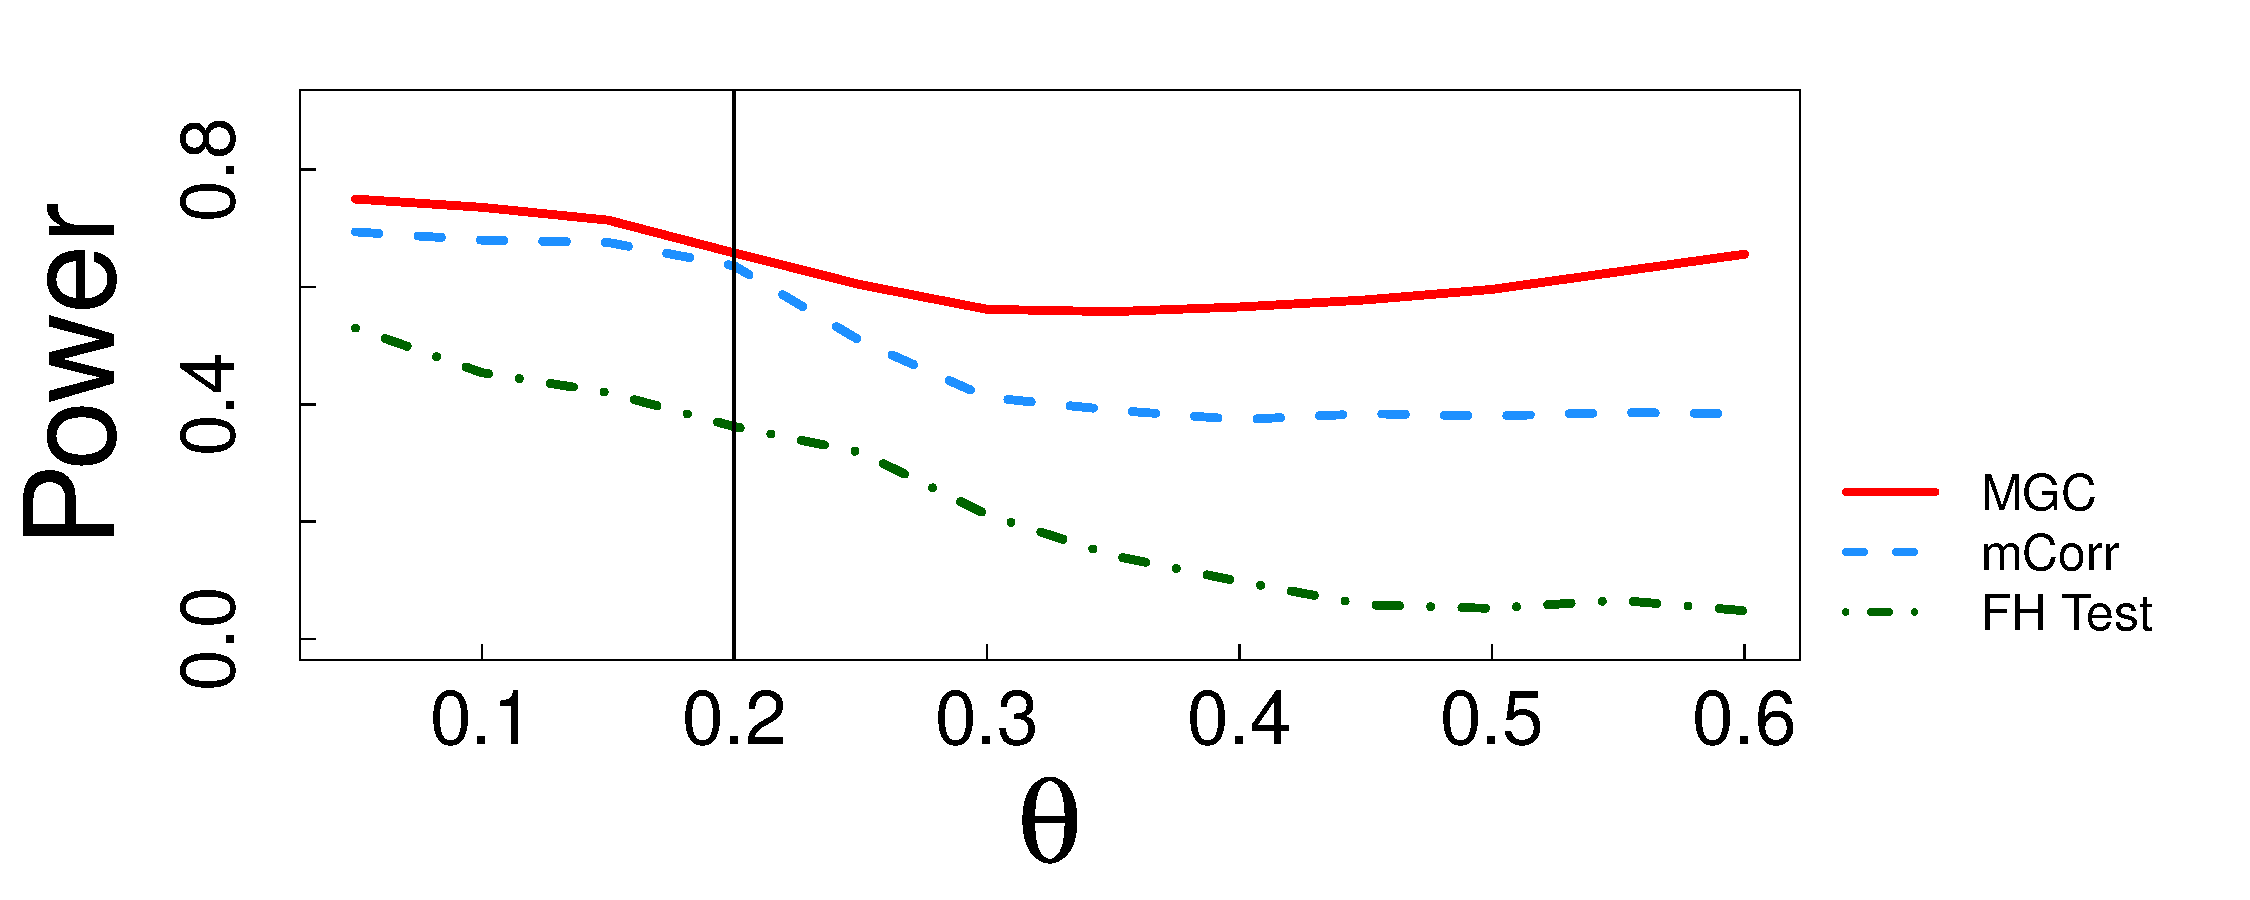
\includegraphics[width=0.7\linewidth]{../Figure/mono_simple.pdf}
	\caption{X-axis of $\theta$ controls the existence/amount of nonlinear dependency and in this particular case nonlinearity exists when $\theta > 0.2$ and gets larger as it increases. You can see the discrepancy in power between global and local scale tests also gets larger accordingly, mostly due to decreasing power of \texttt{mCorr} or \texttt{FH} test but relatively stable power of \texttt{MGC} under nonlinear dependency.}
	\label{fig:powerplot}
\end{figure}

% degree-corrected two block model
On the other hand, the SBM connotes that all nodes within the same block have the same expected degree. Thus, this block model is limited by homogeneous distribution within block and provides a poor fit to networks with highly varying node degrees within block or community. Instead the Degree-Corrected Stochastic Block model (DCSBM) proposed by \cite{karrer2011stochastic} add another random variable associated with each node to vary the node degrees. In the model~\ref{eq:tau}, we controlled the amount of such variability by $\tau$; the larger the value $\tau$ is, the more variability degree or edge distribution has. In Figure~\ref{fig:dcSBM}, power based on Euclidean distance of $\mathbf{A}$ or that of estimated network factors (locations) becomes less sensitive as $\tau$ increases. Compared to these two, diffusion maps are more robust to such variability. 
\vspace*{-0.4cm}
\begin{equation}
E( A_{ij} | \mathbf{X}, \mathbf{V} )  = 0.2 V_{i} V_{j} \cdot I ( |X_{i} - X_{j}| = 0 ) + 0.05 V_{i} V_{j} \cdot I(|X_{i} - X_{j}| = 1),
\label{eq:tau}
\vspace*{-0.4cm}
\end{equation} 
where $X_{i} \overset{i.i.d.}{\sim} Bern(0.5);  V_{i} \overset{i.i.d}{\sim} Uniform(1 - \tau, 1 + \tau), i = 1, \ldots, 250.$
\begin{figure}[ht]
	\centering
	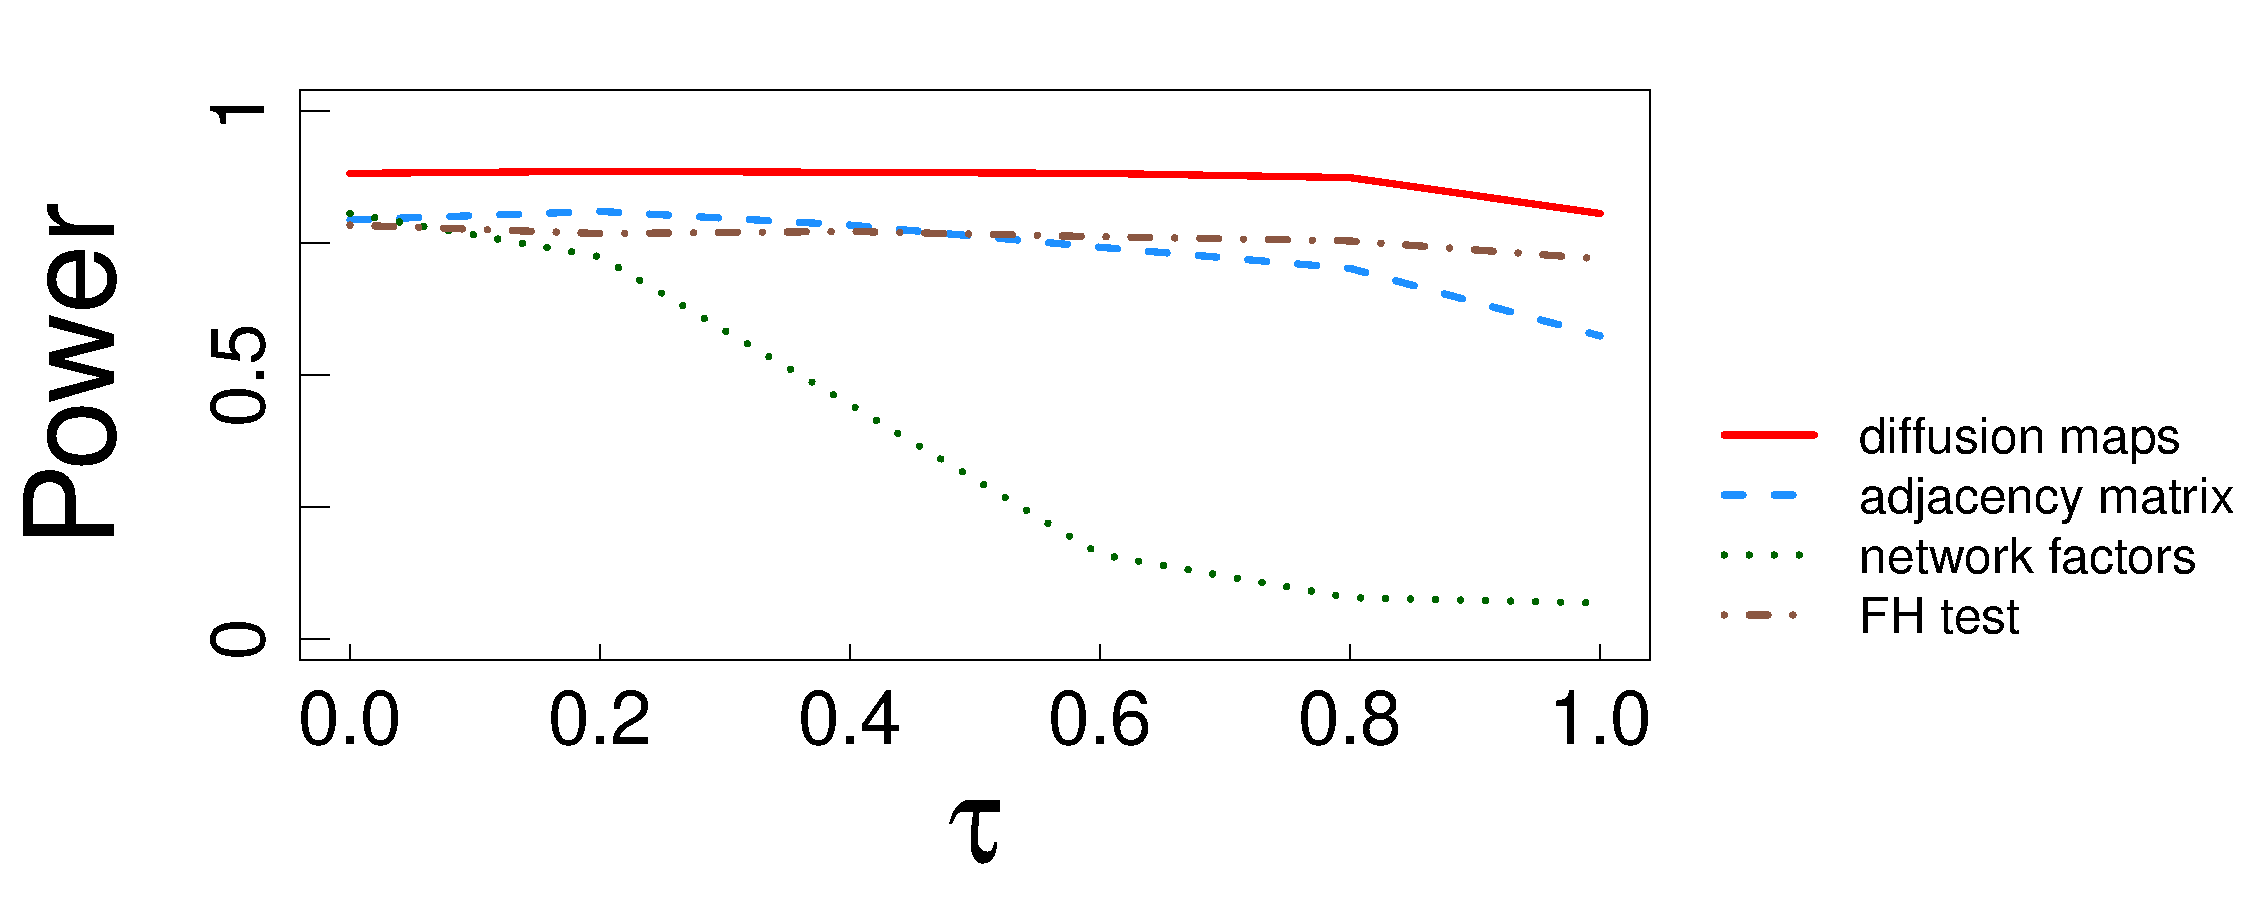
\includegraphics[width=0.7\linewidth]{../Figure/tau_simple.pdf}
	\caption{In degree-corrected SBM where the variability in degree distribution increases as $\tau$ increases, testing power of diffusion maps are more likely to be robust against increasing variability compared to other network metrics, e.g. adjacency matrix or latent positions. \texttt{FH} test statistics allowing different dimensions of network factors perform consistently well but still have less power than \texttt{MGC}.}
	\label{fig:dcSBM}
	\vspace*{-0.5cm}
\end{figure}	

\subsection{Node Contribution Test}
\label{ssec:node}
\begin{figure}[ht]
	\centering
	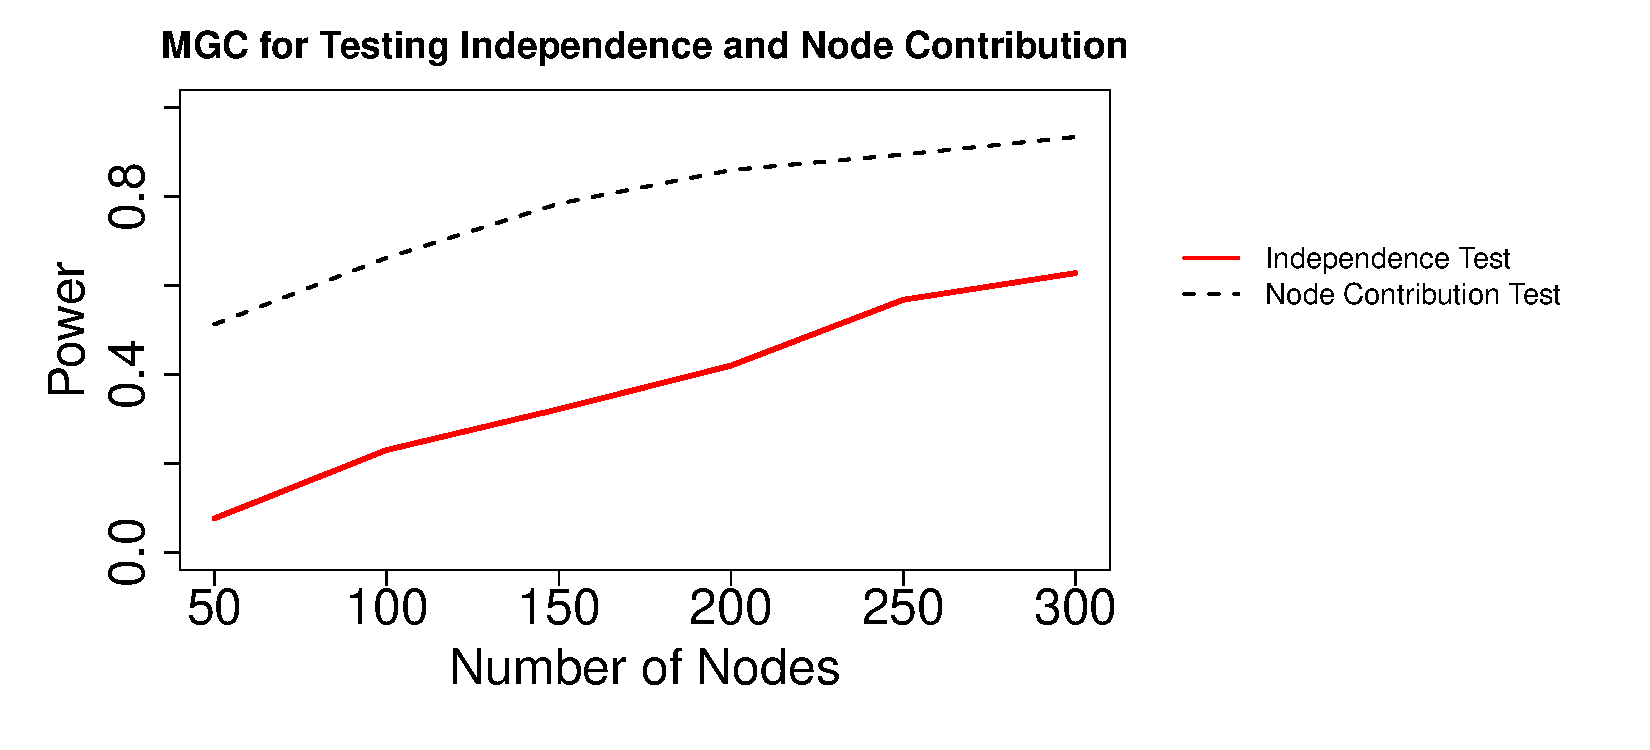
\includegraphics[width=0.7\linewidth]{../Figure/nodecontri.pdf}
	\caption{This plot describes that both power of \texttt{MGC} and the rate of correctly-ranked node contribution increase as the number of nodes increases when only half of the nodes for each simulation actually are set to be dependent on network, which validates the use of node contribution measure in independence test.}
	\label{fig:contribution}
\end{figure}
To examine the effectiveness of node contribution measure in testing dependency as presented in the statistic~\ref{eq:contribution}, we deliberately simulate the network and its nodal attributes as half of the nodes are independent while the other half are dependent on network (model~\ref{eq:contri}). 
\begin{equation}
\begin{gathered}
\begin{aligned}
	& X_{i} \overset{i.i.d}{\sim}  Bern(0.5)  \quad i = 1, \ldots ,n/2, \ldots, n \\
	& E( A_{ij} | X_{i}, X_{j} )   \stackrel{d}{=} \left\{  \begin{array}{cc} 0.4 I(|X_{i} - X_{j}| = 0)  + Bern(0.1) I(|X_{i} - X_{j}| > 0) & i = 1,\ldots,n/2 \\   0.25  & i=1+n/2, \ldots, n  \end{array} \right.
	\end{aligned}
	\end{gathered}
\label{eq:contri}
\end{equation}
As an ad hoc test of node contribution, we rank the nodes in terms of decreasing order of $c(v)$ and count the ratio of dependent samples's ranks within the number of dependent nodes. If it works perfectly, all dependent nodes would take higher rank than every independent node so thus the rate equals to one. We call this rate as \textit{inclusion rate}:
\begin{equation}
\mbox{ inclustion rate}\big(  c(v) \big) = \sum\limits_{v \in V(\mathbf{G})} \big\{  rank_{c(v)}\big(  v \big)  \leq  m  \big\}   /  m,
\label{eq:inclusion_rate}
\end{equation}
where $m (\leq |V(\mathbf{G})|)$ is the number of nodes under network dependence. We set $m=n/2$ out of $n = |V(\mathbf{G})|$.

%%%%%%%%%%%%%%%%%%%%%%%%%%%%%%%%%%%%%%%%%
\section{Real Data Examples}
\label{sec:real}
\begin{figure}[ht]
	\centering
	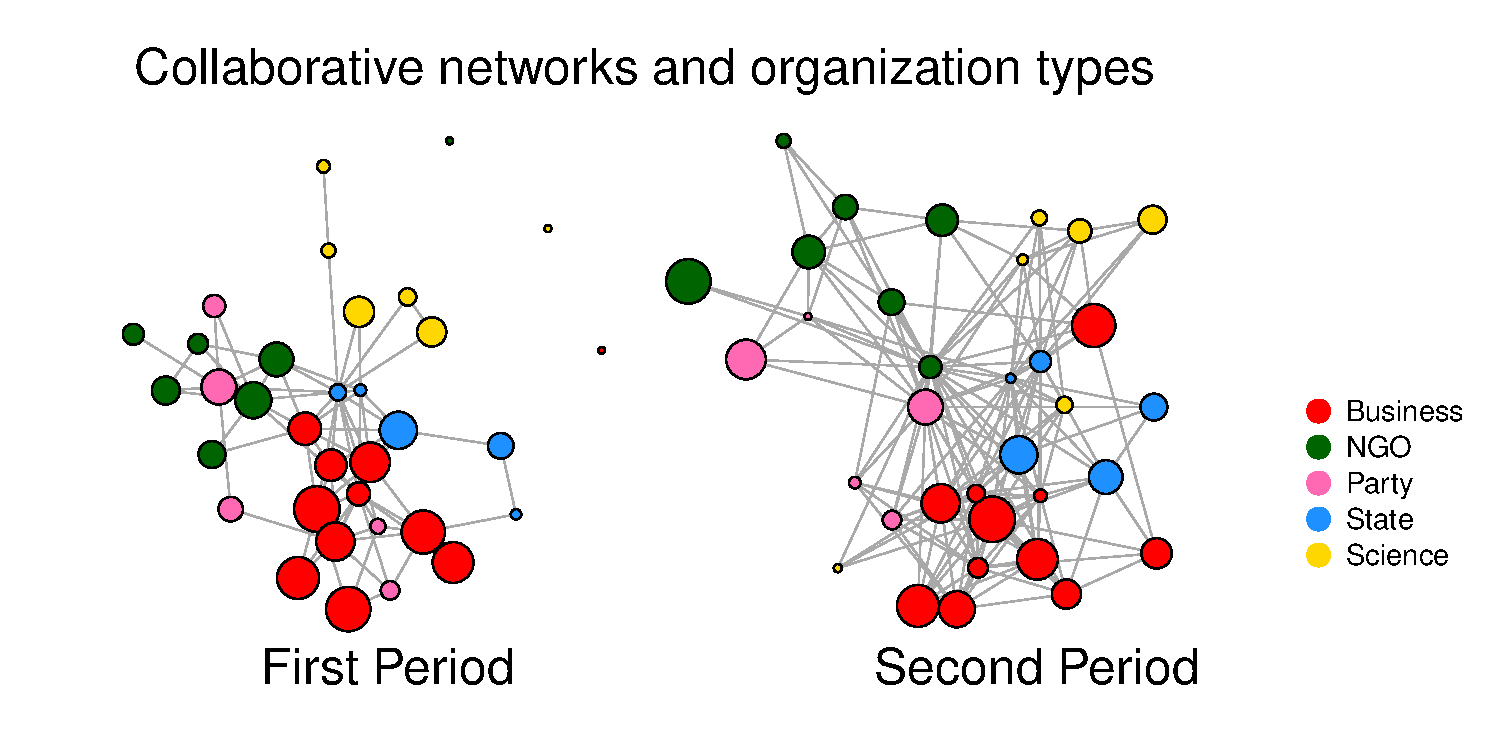
\includegraphics[width=\linewidth]{../Figure/two_politics.pdf}
	\caption{Both panels depict the collaborative networks during the two time periods having significant network dependency in types of organizations. Using \texttt{MGC} statistics, we are not only able to test network independence but also calculate each node's amount of contribution to detecting dependence, which is proportional to node size here. You can tell that the tendency to collaborate within the same type is strongest among the business group while scientist relatively collaborates less with any others, especially in the first period.}
	\label{fig:politics}
\end{figure}
In the field of political science, who exerts more powerful impacts than the others over political network and which factors impact on the power differentials are one of the interests~\citep{ingold2014structural}. \cite{minhas2016inferential} made an inference from political networks~\citep{cranmer2016navigating} via the additive and multiplicative effects (AME). The AME model estimates the latent factors and uses them to test independence with the nodal attributes. Among diverse attributes that \cite{cranmer2016navigating} provided, we focus on the types of organizations and how 34 political organizations having different types are participating policy network. We changed a given directed network into undirected network and use a dissimilarity matrix for distance matrix of the attributes, i.e., $\parallel \mathbf{X}_{i}  - \mathbf{X}_{j} \parallel = 0$ if and only if node $i$ and node $j$ are from the same type and one otherwise. Two collaboration networks comprised of the same set of nodes across two time periods are provided~\citep{ingold2014structural}. Figure~\ref{fig:politics} and Figure~\ref{fig:barplots} illustrates these two networks and shows each node's reliance on its organization type when collaborating. During the two periods, the network independence test statistics of \texttt{MGC} (p-value : (0.002 , 0.002)) and \texttt{dCorr} (p-value : ( 0.000, 0.000)) using diffusion distance matrices result in significant p-values across diffusion times from $t=1$ to $t=10$. The conclusion from the \texttt{FH} test (p-value : ( 0.000, 0.000)) is also the same.  
\begin{figure}[ht]
	\centering
	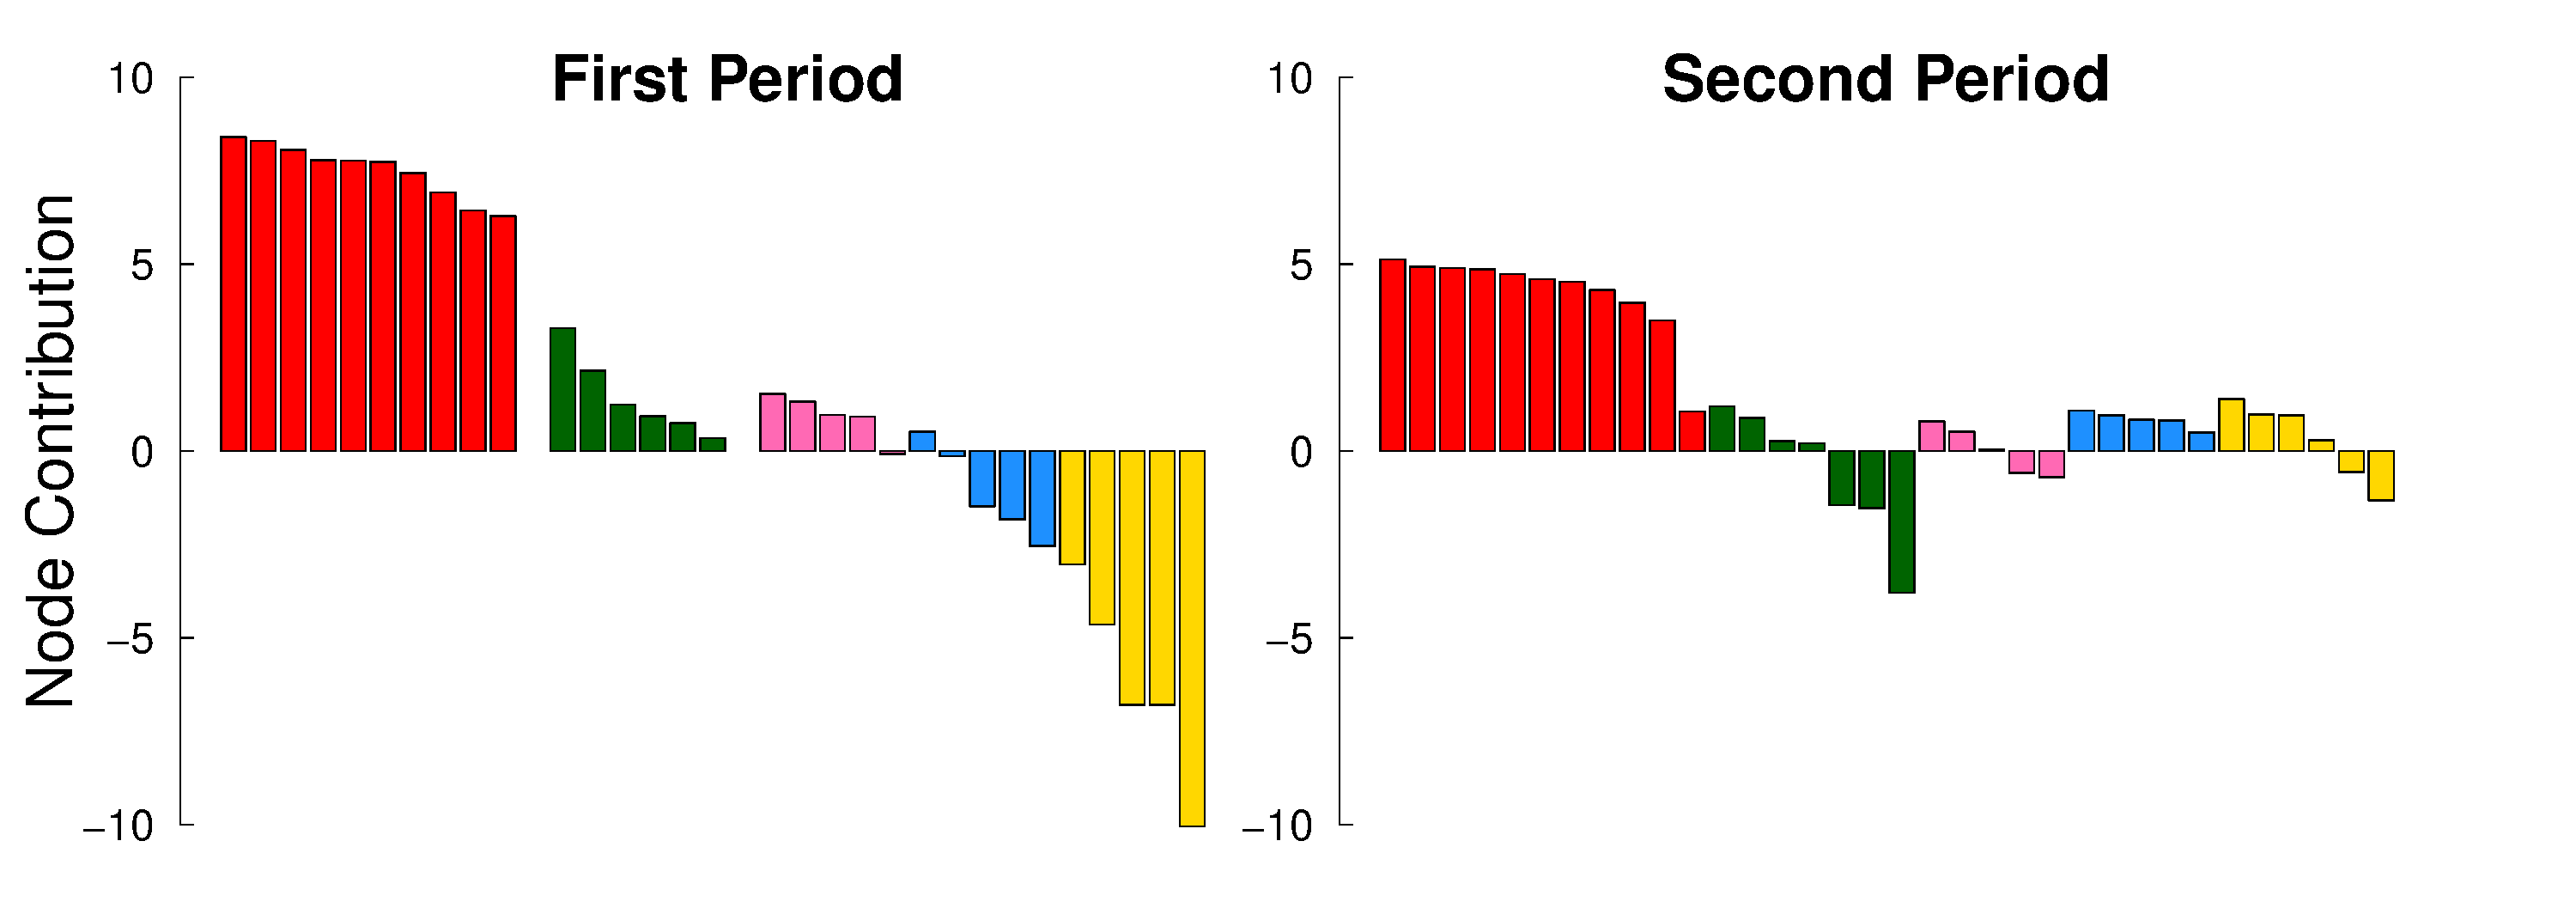
\includegraphics[width=\linewidth]{../Figure/barplots_nolegend.pdf}	
	\caption{In the first period, we have two extreme cases among the business group and science group, which reflects our observations in Figure~\ref{fig:politics}. Generally organizations cooperate more actively between different types in the second period but still their collaboration network is highly dependent on their organization types especially for business group.}
	\label{fig:barplots}
\end{figure}


%%%%%%%%%%%%%%%%%%%%%%%%%%%%%%%%%%%%%%%%
\vspace*{-0.5cm}
\section{Conclusion}
\label{sec:conc}
	\vspace*{-0.2cm}
In this paper, we convince that \texttt{MGC}, merged with a family of diffusion distance, provides us powerful independence test statistics in network. Having multiscale statistics, i.e.~one parameter family of statistics, is not avoidable because we regard distance between the nodes over network as a dynamic process. Through simulation studies, we demonstrate that our methods perform better than the others especially under nonlinear dependency, and we are able to measure each node's contribution to detecting dependency. Deriving the contributions is particularly important when there have possibly different amounts of the dependencies among the nodes.  

However obtaining a full family of statistics are computationally infeasible. Also we did not suggest any theoretically supported tools to select one metrics among them so thus we have one single statistic. As an ad hoc, we selected an \textit{optimal} diffusion time $t$ with highest power from $t=1$ to $t=10$ for our simulation since we could observe a stabilized empirical power within this period. Developing the adaptive method to find this optimal $t$ where dependence is maximized would be a natural next step. Despite these shortcomings, we expect that we could also enjoy the properties of \texttt{MGC} and a family of diffusion distances in solving diverse problems which require to utilize local relationship of the data sets. For instance, we might be able to implement independence testing between two networks of same size by using diffusion distance of each network to investigate whether a pair of networks are topologically or structurally independent. This kind of work would shed light on revealing any relationship between the data sets which are not necessarily a random vector.

%%%%%%%%%%%%%%%%%%%%%%%%%%%%%%%%%%%%%%%%%%%%
\vspace*{-0.5cm}
\bibliography{reference}
%\bibliographystyle{plainnat}
%%%%%%%%%%%%%%%%%%%%%%%%%%%%%%%%%%%%%%%%%%%%%%
\vspace*{-0.5cm}
\section{Appendix}
\vspace*{-0.2cm}
\subsection{Lemmas and Theorems}
\label{ssec:proof}

%%%%%%%%%%%%%%%%%%%%%%%%%%%%%%%%%%%%%%%%	
\begin{proof}[\textbf{Proof of Lemma~\ref{main_lemma}}]
	Diffusion map at time $t$ is represented as follows :
	\begin{equation}
	\mathbf{U}_{t}(i) = \begin{pmatrix} \lambda^{t}_{1} \phi_{1}(i) & \lambda^{t}_{2} \phi_{2} (i)  & \cdots & \lambda^{t}_{q} \phi_{q}(i) \end{pmatrix} \in \mathbb{R}^{q}.
	\end{equation}
	where $\Phi = \Pi^{-1/2}\Psi$ and $Q= \Psi \Lambda \Psi^{T} = \Pi^{1/2} P \Pi^{-1/2}$. 
	Thus $P \Pi^{-1/2} \Psi = \Pi^{-1/2} \Psi \Lambda$. 
	Then for any $r$th row ($r \in \{1,2, ... , q \}$, $(q \leq n)$), we can see that $P \phi_{r} = \lambda_{r} \phi_{r}$  where $\phi_{r} = \begin{pmatrix}  \psi_{r}(1) / \sqrt{\pi(1)} &  \psi_{r}(2) /  \sqrt{\pi(2)} & \cdots & \psi_{r}(n) /  \sqrt{\pi(n)}  \end{pmatrix}$.
	Therefore to guarantee exchangeability (or \textit{i.i.d}) of $\mathbf{U}_{t}$, it suffices to show exchangeability (or \textit{i.i.d}) of $P$.
	
	Assume joint exchangeability of $\mathbf{G}$, i.e. $(A_{ij}) \stackrel{d}{=} \big( A_{\sigma(i) \sigma(j)} \big)$. Since $A_{ij}$ is binary, $A_{ij} / \sum\limits_{j} A_{ij} = A_{ij} /  (1 + \sum\limits_{l \neq j} A_{il})$. Moreover, $A_{ij}$ and $(1 + \sum\limits_{l \neq j} A_{il})$ are independent given its link function $g$, and $A_{\sigma(i) \sigma(j)}$ and $(1 + \sum\limits_{l \neq j} A_{\sigma(i) \sigma(l)})$ are independent also given $g$. Then the following joint exchangeability of transition probability holds for $i \neq j; i,j = 1,2, \ldots,n$:	
	\begin{equation}
		\vspace*{-0.2cm}
	\big( P_{ij} \big) = \left(  \frac{A_{ij}}{1 - A_{ij} + \sum\limits_{j=1}^{n} A_{ij} } \right)  \stackrel{d}{=} \left( \frac{A_{\sigma(i) \sigma(j)} }{1 - A_{\sigma(i) \sigma(j)} + \sum\limits_{\sigma(j) = 1}^{n} A_{\sigma(i) \sigma(j)} } \right) = \big( P_{\sigma(i) \sigma(j)} \big)
	\end{equation}
	When $i = j$, $P_{ij} = P_{\sigma(i) \sigma(j)} = 0$ for $i=1,2, \ldots, n$. Thus, transition probability is also exchangeable. This results exchangeable eigenfunctions $\{ \Phi(1), \Phi(2), , ... , \Phi(n) \}$ where $\Phi(i) := \begin{pmatrix} \phi_{1}(i) & \phi_{2}(i) & \cdots & \phi_{q}(i) \end{pmatrix}^{T}$, $i=1,2, \ldots, n$. Thus diffusion maps at fixed $t$, $\mathbf{U}_{t} = \begin{pmatrix} \Lambda^{t} \Phi(1)  & \Lambda^{t} \Phi(2) & \cdots & \Lambda^{t} \Phi(n)  \end{pmatrix}$ are exchangeable. Furthermore by \textit{de Finetti's Theorem}, we can say that $\mathbf{U}(t) = \{ \mathbf{U}_{t}(1), \mathbf{U}_{t}(2), \ldots, \mathbf{U}_{t}(n)    \}$ are conditionally independent on their underlying distribution.
\end{proof}

%%%%%%%%%%%%%%%%%%%%%%%%
\begin{proof}[\textbf{Proof of Theorem~\ref{theoremMain}} Consistency of \texttt{dCorr} applied to exchangeable variables]
	\bigskip
	
	For exchangeable sequence of $(\mathbf{W}, \mathbf{Y}) = \{ (\mathbf{w}_{i}, \mathbf{y}_{i}) ; i = 1,2, \ldots, n \}$ which is identically distributed as $(\mathbf{w}, \mathbf{y})$ with finite second moment,  we have 
	\begin{eqnarray}
	\mathcal{V}_{n}^{2}(\mathbf{W},\mathbf{Y}) &\longrightarrow \mathcal{V}^{2}(\mathbf{w},\mathbf{y}) \quad \quad \mbox{ as } n \rightarrow \infty
	\label{eq:conv1}
	\end{eqnarray}
	where $\mathcal{V}^{2} (\mathbf{w},\mathbf{y}) := \| g_{\mathbf{w},\mathbf{y}}(t,s) - g_{\mathbf{w}}(t) g_{\mathbf{y}}(s) \|^2$, and $g_{\cdot}$ is a characteristic function, e.g., $g_{\mathbf{w},\mathbf{y}}(t,s) = E\{\exp\{i \left\langle t,\mathbf{w} \right\rangle  +i \left\langle  s,\mathbf{y}\right\rangle \}\}$. This follows exactly the same as \textit{Theorem 1} in \cite{szekely2007measuring}. Note that this Lemma always holds without any assumption on $\{(\mathbf{w}_{i},\mathbf{y}_{i}), i=1,2,...,n\}$.


Followed by \textit{de Finetti's Theorem}, if and only if $\{ \mathbf{w}_{i} \}$ are (infinitely) exchangeble, there exists an underlying distribution $f_{\mathbf{w}}$ of $\mathbf{w}$ such that $\mathbf{w}_{i}  \overset{i.i.d}{\sim} f_{\mathbf{w}} $. By the same logic there exists a random, we have an underlying distribution $f_{\mathbf{y}}$ where $\mathbf{y}_{i} \overset{i.i.d}{\sim} f_{\mathbf{y}}$. Let $(\mathbf{w}_{i}, \mathbf{y}_{i}) \overset{i.i.d}{\sim}   f_{\mathbf{w}, \mathbf{y}}$. Then under the assumption of finite second moment of the underlying distributions and measurable, conditioned random functions, we have a strong large number for V-statistics followed by \cite{szekely2007measuring}, i.e., 
\begin{eqnarray}
\displaystyle\int_{D(\delta)}{\|g_{\mathbf{w},\mathbf{y}}^{n}(t,s)-g_{\mathbf{w}}^{n}(t)g_{\mathbf{y}}^{n}(s)\|^{2}}dh &\stackrel{n \rightarrow \infty}{\longrightarrow} 
\displaystyle\int_{D(\delta)}{\|g_{\mathbf{w},\mathbf{y}}(t,s)-g_{\mathbf{w}}(t)g_{\mathbf{y}}(s)\|^{2}}dh,
\label{eq:SLLN}
\end{eqnarray}
where $D(\delta)=\{(t,s):\delta \leq |t|_{p} \leq 1/\delta,\delta \leq |s|_{q} \leq 1/\delta\}$, and $h(t,s)$ is the weight function chosen in \cite{szekely2007measuring}. 	
It follows that 
\begin{eqnarray}
\mathcal{V}_{n}^{2}(\mathbf{W},\mathbf{Y}) &\rightarrow 0 \quad \mbox{ as } n \rightarrow \infty
\label{eq:conv2}
\end{eqnarray}
if and only if $g_{\mathbf{w},\mathbf{y}}(t,s) = g_{\mathbf{w}}(t) g_{\mathbf{y}}(s)$, i.e., $\mathbf{w}$ is independent of $\mathbf{y}$. Therefore, the \texttt{dCorr} or \texttt{mCorr} converges to $0$ if and only if  underlying distributions are independent; and its testing power converges to $1$ under any joint distribution of finite moments. Since the multiscale generalized correlation based on any consistent global correlation is also consistent~\citep{shen2016discovering}, \texttt{MGC} statistic constructed by \texttt{dCorr} or \texttt{mCorr} is also consistent in testing dependence.
\end{proof}
%%%%%%%%%%%%%%%%%%%%%%%%%%5
\begin{proof}[\textbf{Proof of Theorem~\ref{theorem2}} Consistency of \texttt{MGC} applied to exchangeable variables]
	
Under the exchangeability and finite second moment assumptions of underlying distribution, $\mathcal{V}^{2}_{n}(\mathbf{W},\mathbf{Y}) \xrightarrow{n \rightarrow \infty}  0$ if and only if underlying distribution of $\{\mathbf{w}_{i} \}$, $f_{\mathbf{w}}$ is independent from underlying distribution of $\{ \mathbf{y}_{i}  \}$, $f_{\mathbf{y}}$. Now suppose that we have undirected, connected network $\mathbf{G}$ with a family of diffusion maps $\{ \mathbf{u}_{t}  \}$ and with nodal attributes $\{ \mathbf{x}  \}$. We have shown in the Lemma~\ref{main_lemma} that $\{ \mathbf{u}_{t}  \}$ are exchangeable for each $t \in \mathbb{N}$. Thus there exists an underlying distribution of $\mathbf{u}_{t}$ such that $\mathbf{u}_{t}(i) \overset{i.i.d}{\sim} f_{\mathbf{u}^{(t)}}$ for each of $t= 1,2,\ldots $; and we have $\mathbf{x}_{i} \overset{i.i.d}{\sim} f_{\mathbf{X}}$. Under the assumption of finite second moment of $\mathbf{u}^{(t)}$ and $\mathbf{x}$, \texttt{MGC} statistics constructed by $\{  (  \mathbf{u}_{t}(i), \mathbf{x}_{i} ) : i = 1,2,\ldots, n  \}$ yield a consistent testing which determines the independence between underlying distributions of $\mathbf{u}^{(t)}$ and $\mathbf{x}$. From the same setting of network $\mathbf{G}$, we have estimated \textit{i.i.d} node-specific network factors $\{ \mathbf{F}_{i} \}$ so that $n$-pair of \textit{i.i.d} $\{ ( \mathbf{F}_{i}, \mathbf{x}_{i} )  \}$ can be applied to \texttt{MGC} or other distance-based tests without assuming conditioning underlying distribution. In case of using adjacency matrix directly into test, we must assume that the adjacency matrix comes from connected directed network, i.e. $A_{ij} \overset{i.i.d}{\sim} f_{A}$ for all $i,j=1,2,\ldots, n$; otherwise, each column is dependent on one another.  
\end{proof}

\end{document}